\section{Difa Al Fansha(1174076)}
\subsection{Pengertian}
\begin{itemize}
	\item \textbf{Geografi} \\
	'Merupakan ilmu yang melukiskan dan menggambarkan keadaan bumi.' \\ 
(Erastoshenes, 200SM). \\ 
Geografi biasa disebut juga dengan spasial, geografi sangat berkaitan dengan peta, karena peta adalah gambaran sebuah lingkungan. Dalam peta, simbol, warna dan gaya garis digunakan sebagai perwakilan dari setiap spasial yang berbeda pada peta poligon (2-D) dan permukaan (3-D)
	
	\item \textbf{Informasi} \\
Pengolahan sejumlah data (gambar, suara, text, dan lain sebagainya). Semua data harus diasosiasikan pada object spasial yang mampu mmebuat peta menjadi cerdas (intelligent).

	\item \textbf{Sistem} \\
Kumpulan elemen-elemen yang saling  berhubungan dalam sebuah lingkungan yang dinamis untuk mencapai tujuan tertentu.
	
	\item \textbf{Kesimpulan :} \\
Sistem geografi adalah sebuah komputer yang berbasis sistem informasi digunakan untuk memberikan informasi bentuk digital dan analisa terhadap permukaan georafi bumi.\\
Definisi dari sistem informasi geografis dapat selalu berubah-ubah, karna sig merupakan bidang kajian ilmu dan teknologi yang masih baru.

\end{itemize}

\subsection{Link}
https://youtu.be/2SusnHVlTYA

\subsection{Plagiarism}
\begin{figure}[H]
	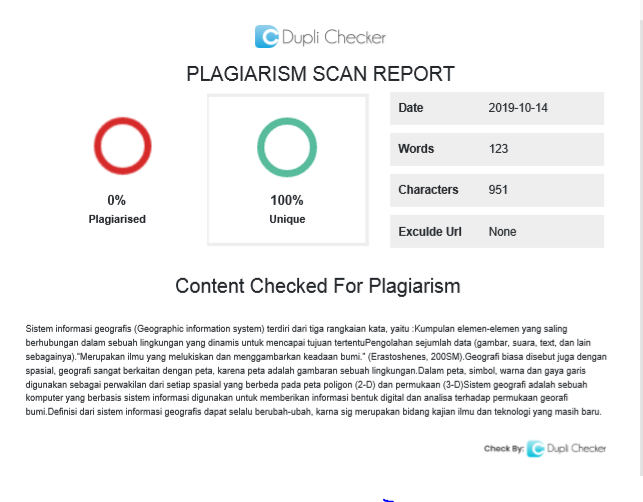
\includegraphics[width=8cm, height=8cm]{figures/Tugas1/1174076/1174076.png}
	\centering
	\caption{Gambar Plagiarisme 1174076}
\end{figure}